\documentclass[UTF8]{ctexart}
\usepackage{subfigure}
\usepackage{caption}
\usepackage{amsmath}
\usepackage{geometry}
\usepackage{graphicx}
\usepackage{gensymb}
\usepackage{wrapfig}
\usepackage{titlesec}
\usepackage{float}
\usepackage{diagbox}
\usepackage{fancyhdr}
\pagestyle{plain}
\geometry{a4paper,scale=0.8}
\CTEXsetup[format+={\raggedright}]{section} 
\title{量统2016-2017郭永期末}
\author{Deschain}
\titlespacing*{\section}
{0pt}{0pt}{0pt}
\titlespacing*{\subsection}
{0pt}{0pt}{0pt}
\titlespacing*{\paragraph}
{0pt}{0pt}{0pt}
\titlespacing*{\subparagraph}
{0pt}{0pt}{0pt}
\titleformat*{\section}{\normalsize}
\begin{document}
\maketitle
\section*{一、}
1.近独立粒子系统:系统的粒子间的相互作用的平均能量远小于单个粒子的平均能量。\\
2.玻尔兹曼关系:$S=kln(W\{n_i\})$,S是熵,k是Boltzmann常数,$W\{n_i\}$是系统的微观状态数。\\
3.等几率原理:对于处于平衡态的孤立系统,各个微观态出现的几率相等。\\
4.固体Einstein模型:有N个原子的固体,振动自由度为3N,假设3N个振子的振动频率都是$\nu$,振子彼此独立。\\
5.准粒子:具有粒子属性而无粒子实体的粒子。
\section*{二、}
1.
\begin{equation*}
  \begin{aligned}
    W\{n_i\}=\prod\limits_i\frac{g_i!}{n_i!(g_i-n_i)!}
  \end{aligned}
\end{equation*}
2.
\begin{equation*}
  \begin{aligned}
     & ln(W\{n_i\})\approx\sum\limits_i g_ilng_i-n_ilnn_i+(n_i-g_i)ln(g_i-n_i)         \\
     & F(n_i)=ln(W\{n_i\})+\alpha(N-\sum n_i)+\beta(E-\sum n_i\varepsilon_i)           \\
     & \frac{\partial F}{\partial n_i}=ln(\frac{g_i}{n_i}-1)-\alpha-\beta\varepsilon_i \\
     & n_i=\frac{g_i}{e^{\alpha-\beta\varepsilon_i}+1}
  \end{aligned}
\end{equation*}
3.
\begin{equation*}
  e^\alpha>>1
\end{equation*}
\section*{三、}
\begin{equation*}
  \begin{aligned}
     & \varepsilon_i=\varepsilon_t+\varepsilon_\alpha^l+U
    =\frac{p_x^2+p_y^2}{2m}+\varepsilon_\alpha^l+U                                        \\
     & n(p_x,p_y)dp_xdp_y=\frac{1}{h^2}e^{-\alpha-\frac{\beta}{2m}(p_x^2+p_y^2)}dp_xdp_y
    \int e^{-\beta U}dxdydz\sum\limits_ag_a^le^{-\beta\varepsilon_a^l}                    \\
     & N=\frac{1}{h^2}\int e^{-\alpha-\frac{\beta}{2m}(p_x^2+p_y^2)}dp_xdp_y
    \int e^{-\beta U}dxdydz\sum\limits_ag_a^le^{-\beta\varepsilon_a^l}                    \\
     & =\frac{e^{-\alpha}2\pi m}{h^2\beta}
    \int e^{-\beta U}dxdydz\sum\limits_ag_a^le^{-\beta\varepsilon_a^l}                    \\
     & n(p_x,p_y)dp_xdp_y=\frac{N\beta}{2\pi m}e^{-\frac{\beta}{2m}(p_x^2+p_y^2)}dp_xdp_y \\
     & n(p)dp=\int_0^{2\pi}\frac{N\beta}{2\pi m}pe^{-\frac{\beta}{2m}p^2}dpd\theta
    =\frac{N\beta}{m}pe^{-\frac{\beta}{2m}p^2}dp                                          \\
     & n(v)dv=Nm\beta e^{\frac{mv^2}{2kT}}vdv
    =2\pi N\frac{m}{2\pi kT}e^{\frac{mv^2}{2kT}}vdv                                       \\
  \end{aligned}
\end{equation*}
\section*{四、}
1.
\subsection*{}
\begin{wrapfigure}{r}{3cm}
  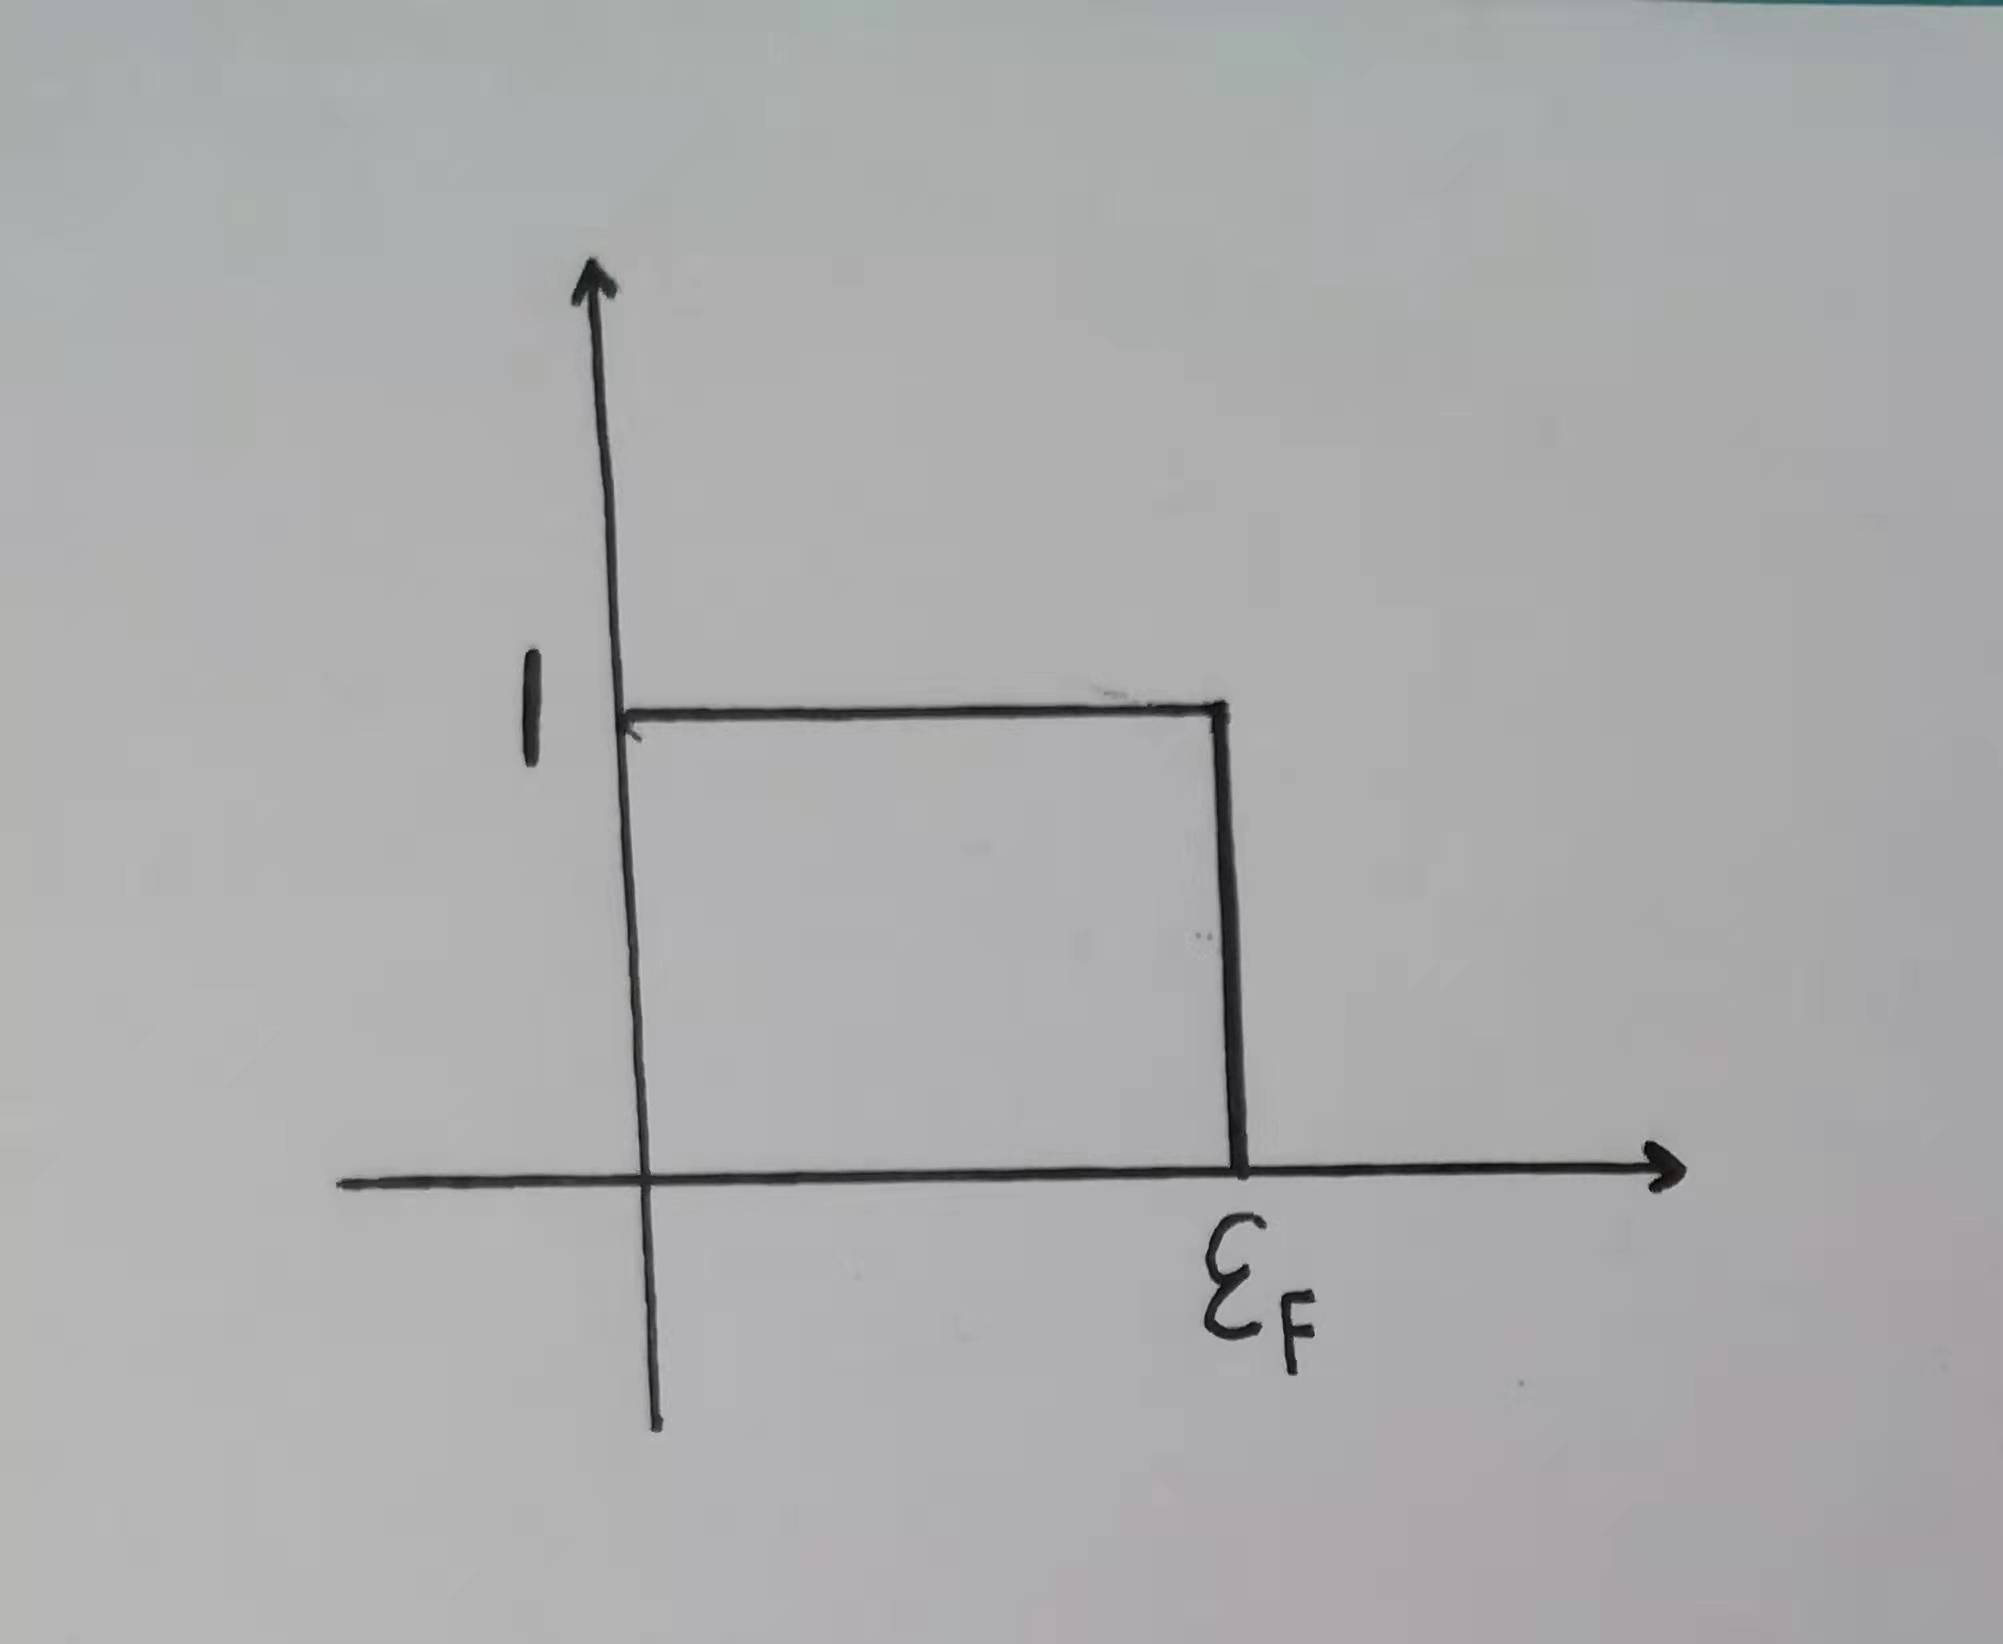
\includegraphics[width=3cm]{4_1.jpg}
\end{wrapfigure}
$T=0K$时,$\varepsilon_F$以下的能级完全填满,$\varepsilon_F$以上的能级完全空着。
\begin{equation*}
  f=\begin{cases}
    1,\quad\quad 0<\varepsilon<\varepsilon_F \\
    0, else
  \end{cases}
\end{equation*}
2.
\subsection*{}
\begin{wrapfigure}{r}{3cm}
  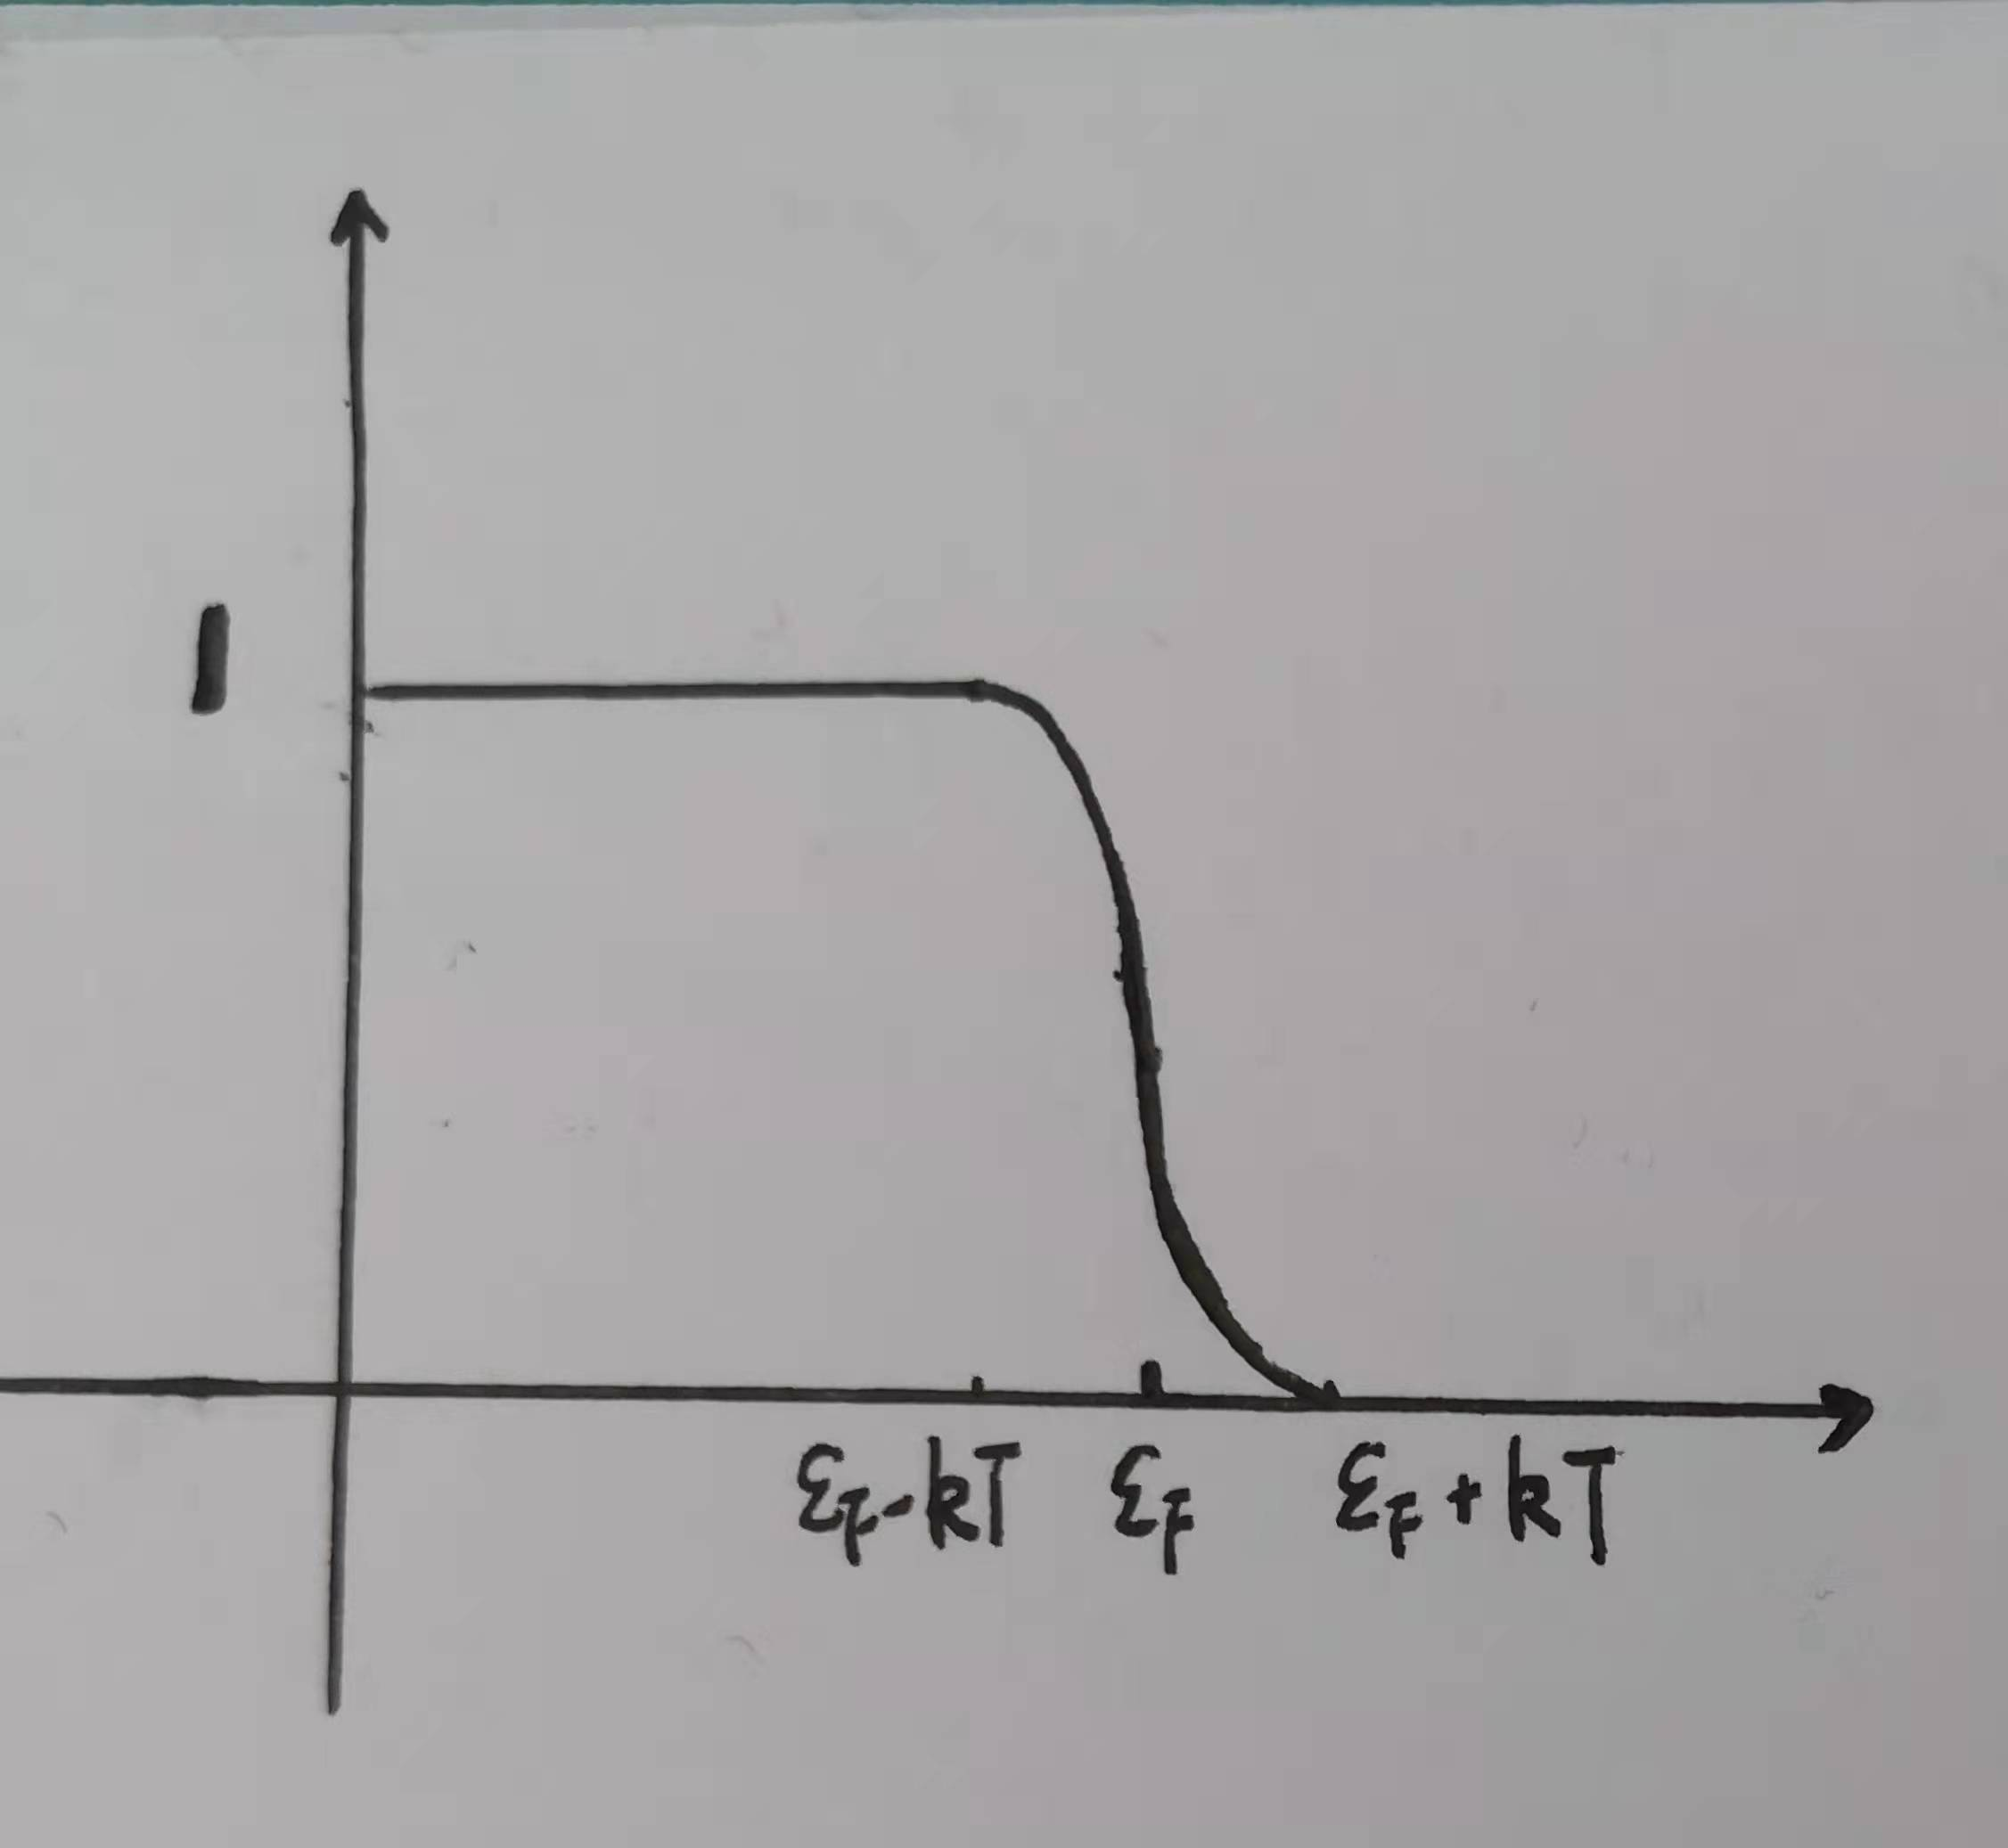
\includegraphics[width=3cm]{4_2.jpg}
\end{wrapfigure}
$T>0K$时,通常的温度$T<<T_F$,
\begin{equation*}
  f=\begin{cases}
    1,\quad\quad\quad 0<\varepsilon<\varepsilon_F-kT            \\
    0\sim1, \quad \varepsilon_F-kT<\varepsilon<\varepsilon_F+kT \\
    0,\quad\quad\quad,else
  \end{cases}
\end{equation*}
3.
\subsection*{}
\begin{equation*}
  \begin{aligned}
     & N=\int_0^{\varepsilon_F}g(\varepsilon)d\varepsilon
    =\int_0^{\varepsilon_F}\frac{4\pi V(2m)^\frac{3}{2}\sqrt\varepsilon d\varepsilon}{h^3}
    =\frac{8\pi V}{h^3}(2m\varepsilon_F)^\frac{3}{2}            \\
     & \varepsilon_F=\frac{h^2}{2m}(\frac{3N}{\pi})^\frac{2}{3}
  \end{aligned}
\end{equation*}
\section*{六、}
1.当温度从$T_c$开始下降时,基态上的粒子数迅速增加,与总粒子数具有相同的量级。$T=0K$时,
全部粒子集中在基态上。\\
一个量子态上可以容纳多个Bose子,但只能容纳一个Fermi子。\\
2.\\
二维:
\begin{equation*}
  g(\varepsilon)=\frac{2\pi JSm}{h^2},\quad
  N=\int_0^\infty\frac{g(\varepsilon)d\varepsilon}{e^\frac{\varepsilon-\mu}{kT}-1}
\end{equation*}
积分发散,故无法凝聚。\\
一维:
\begin{equation*}
  g(\varepsilon)=JL\sqrt{\frac{2m}{\varepsilon}},\quad
  N=\int_0^\infty\frac{g(\varepsilon)d\varepsilon}{e^\frac{\varepsilon-\mu}{kT}-1}
\end{equation*}
积分发散,故无法凝聚。

\end{document}